\chapter{Dry sand mining}
%\section{River bank instability due to sand mining}
%Much like the Paraná Guazú, sand mining is a relevant topic in the lower Mekong river. Previous studies have shown that incision due to the sand mining exists in this river and is of the order of 0.13 m per year \autocite{brunierRecentMorphologicalChanges2014}. \citeauthor{hackneyRiverBankInstability2020} showed that this river bed lowering not only has morphological consequences but also geotechnical ones, since a lower river bed can cause instability of the river banks.

%In the previous study it was found that, even in conservative scenarios, entire sections of river banks along the lower Mekong River would shift from a stable to a seasonally unstable condition. This means they are likely to fail during periods of heavy rainfall. In more extreme scenarios with more sand mining, the researchers found that 63\% of river banks would become seasonally unstable \autocite{hackneyIncreasedHydraulicRoughness2025}.

%In this chapter, the potential risks of river bank instability due to sand mining in the Paraná Guazú-river are investigated.

\section{Oil and gas mining in Argentina}
For much of its history, Argentina was regarded as a modest oil producer, struggling to meet its own energy demands. This perception shifted with the 2011 discovery of the Vaca Muerta shale formation, located in the Neuquén basin in Patagonia. The Argentine energy company YPF identified approximately 150 million barrels of recoverable oil in the field, which was regarded as a new source of hope for economic stability by the president \autocite{kraussArgentinaHopesBig2011}.

The discovery was followed by significant foreign investment from companies such as Total, ExxonMobil, Apache, and EOG Resources. More exploration was done and now it is clear that Argentina possesses the world’s fourth-largest shale oil and second-largest shale gas reserves. The Government of Argentina still views the oil and gas sector as a crucial part of its economy, by driving exports as well as generating foreign currency \autocite{internationaltradeadministrationArgentinaCountryCommercial2025}.

The Nuequén basin is located in the provinces of Neuquén, Mendoza, and Río Negro in the South of Argentina and has been an important basin for oil and gas since more than a century. Production started in 1918 and in 2004, 45\% of Argentinian oil production and 61\% of its gas production came from this area \autocite{u.s.energyinformationadministrationTechnicallyRecoverableShale2013}. This was done through conventional methods, but after the discovery of the Vaca Muerta shale basin, fracking has become increasingly important for the region and the country.

The Vaca Muerta shale consists of finely-stratified black to dark grey shale and lithographic lime-mudstone and is 60 to 520 m thick. Estimates are that the formation contains 16 billion barrels of technically recoverable oil and 8722 billion cubic metres of technically recoverable gas \autocite{u.s.energyinformationadministrationTechnicallyRecoverableShale2013}.

As can be seen in figure \ref{fig:oilgasprod}, oil production in Argentina has been steadily increasing since 2020, driven by increased production of the Vaca Muerta formations. After the exploration in 2010, oil from Vaca Muerto as a share of total Argentinian oil production has increased from virtually 0\% to 55\% today. Further, Vaca Muerta now accounts for 47\% of gas supply (PPT) \autocite{internationaltradeadministrationArgentinaCountryCommercial2025}. Since Vaca Muerta is a shale reservoir, all oil and gas from this deposit is extracted by fracking.

\begin{figure}[H]
    \centering
    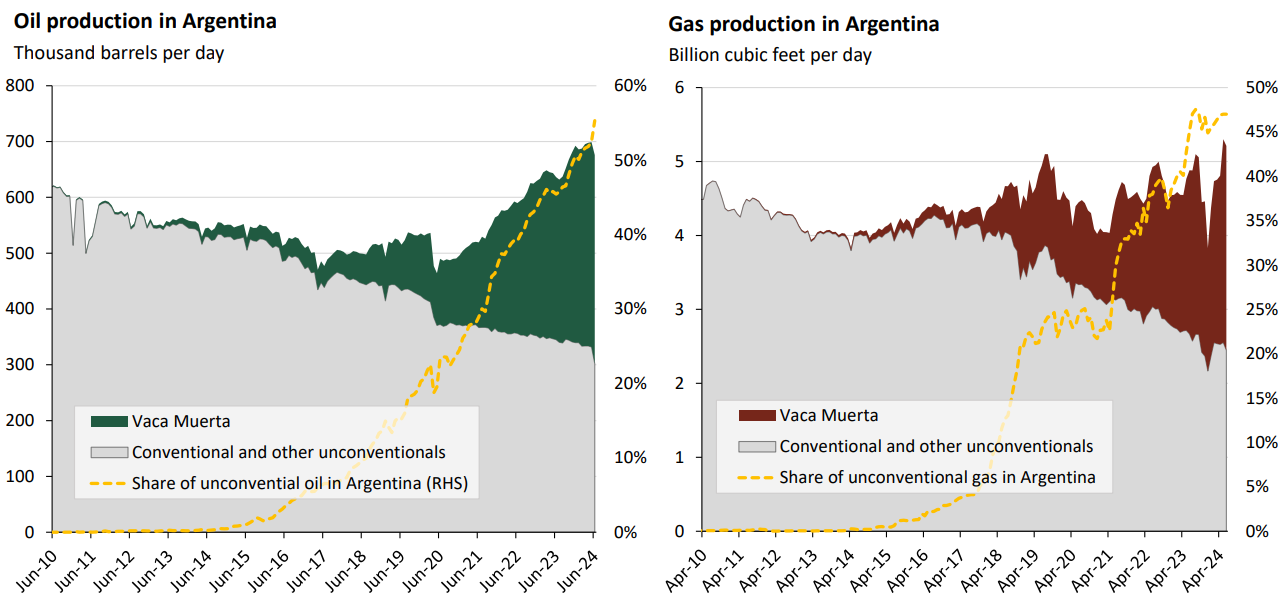
\includegraphics[width=1\linewidth]{figures/ch9/oilgasproduction.png}
    \caption{Oil and gas production in Argentina \autocite{internationaltradeadministrationArgentinaCountryCommercial2025}}
    \label{fig:oilgasprod}
\end{figure}

The numbers in \ref{fig:oilgasprod} help explain why fracking in the Neuquén basin is viewed as crucial to the development of Argentina's economy. It also becomes clear that, considering the volumes present in the reserves, even more gas and oil could still be extracted.

\section{Fracking practices}
In the 1970's, geologists became increasingly aware that large volumes of gas existed in low-permeability sandstones. However, conventional methods did not allow for economic extraction of gas from these `tight reservoirs' \autocite{lawGasTightReservoirs1992}. Hydraulic fracturing, or fracking, a method first tested in 1947 and applied on a large scale for the first time in the 1970's, is a modern method used to extract oil and natural gas from these low-permeability rock formations, such as shale \autocite{melissadenchakFracking1012019}.

The technique begins by drilling a long vertical well. As soon as the desired rock formation is reached, drilling gradually turns horizontal and steel pipes called `casings' are inserted into the well. Small holes are perforated in the casing and then fracking fluid is pumped in at a pressure high enough to create new fractures or open existing ones in the surrounding rock. This allows previously unavailable oil or gas to flow to the surface \autocite{melissadenchakFracking1012019}.

The fracking fluid contains as much as 97 percent water, but also always contains proppants. These are small, solid particles that keep the fractures in the rock formation open after the pressure from injection is removed. Sand is the most widely-used proppant in the fracking industry \autocite{melissadenchakFracking1012019}. Sand is thus an essential substance to keep the drilled pores open and to allow for the fossil fuels to flow out.

Volgens schattingen van geograaf Grosso was tussen 2009 en 2022 86 % van de
gebruikte zand van nationale oorsprong. Van de bijna 8,8 miljoen ton werd iets meer dan 7,4
miljoen ton gewonnen op Argentijns grondgebied, tegenover 1,4 miljoen ton die werd
geïmporteerd.

In 2017, toen de bevolking erin slaagde de anti-frackingwet aangenomen te krijgen om de
watervoerende lagen te beschermen, leverde Entre Ríos al de helft van het silicazand dat in de
Patagonische formatie werd gebruikt. Vandaag ligt dat cijfer tussen 65 % en 75 %.

Van alle departementen waar het bedrijf actief is, is Ibicuy de plaats waar de "boom
van Vaca Muerta" het meest voelbaar is. Bronnen die voor dit artikel zijn geraadpleegd,
schatten dat er dagelijks 350 vrachtwagens uit dit gebied in het zuiden van Entre Ríos
vertrekken. De gemeente zelf voorspelde dat er in 2022 meer dan 1.250.000 ton zand naar
het stroomgebied van Neuquén zou worden vervoerd. Dit is meer dan de totale nationale
winning in 2018.

In Ibicuy zijn onder andere Cristamine, Aresil S. A., YPF, La Chola II, NRG Argentina,
San Marcos Trading en QSand actief. De eerste vier hebben wasinstallaties. Oorspronkelijk
leverden sommige van hen alleen aan de keramiek- en glasindustrie. Tegenwoordig leveren
bedrijven als Aresil hun volledige productie aan de oliesector. La Chola II, met een halve eeuw
ervaring in de winning van riviersand, sloot zich in 2016 aan bij het Vaca Muerta-circuit. Met de
steengroeve Silicatos Islas del Ibicuy en een modulaire fabriek met Ierse technologie die "in
slechts zes dagen" werd geïnstalleerd, wint, wast, sorteert en verzendt het zand voor YPF, zijn
belangrijkste klant(22) .

Maar niet alleen nationale bedrijven hebben belangen in de steengroeven van Entre Ríos. De Belgische Jan de Nul Group, gespecialiseerd in haven- en maritieme engineering, richtte in 2016 Arenas Argentinas del Paraná
op. Volgens eigen zeggen exploiteert het sinds 2019 een steengroeve aan de oever van de rivier El Salto in Diamante, drie kilometer van de plaats Aldea Brasilera en dertig kilometer ten zuiden van de stad Paraná. Daar wint het bedrijf zand met een zuiverheid van bijna 100 %, dat vervolgens in zijn fabriek in dezelfde plaats wordt verwerkt en aan klanten zoals Tecpetrol wordt verkocht.

In de afgelopen twee jaar, 2017 en 2018, was 74% van de totale productie van siliciumzand afkomstig uit Entre Ríos en 26% uit Chubut.
Plaatje
Import

De totale export van siliciumzand en kwartszand vertegenwoordigt minder dan 1% van de import van dezelfde aggregaten in 2018. De bestemmingen zijn buurlanden: Paraguay, Uruguay, Bolivia en Chili, en in alle gevallen wordt voor transport per vrachtwagen gekozen.


Hoewel de vraag naar siliciumzand verspreid is over verschillende industrieën, is de drijvende kracht achter deze vraag de exploitatie van onconventionele olie. Verwacht wordt dat deze trend zich zal doorzetten, niet alleen vanwege de eisen van het project in Neuquén, maar ook vanwege andere soortgelijke projecten die zich nog in de exploratiefase bevinden

Transport:
Weg
Weg + spoor

Het nationale zand dat in Vaca Muerta wordt gebruikt, wordt momenteel vervoerd door vrachtwagens die minstens 1300 km afleggen vanuit Entre Ríos. De steengroeven liggen ver van de vindplaatsen. Wegtransport maakt overslag overbodig en bovendien rijdt de vrachtwagen sneller dan de andere vervoersmiddelen. De vrachtwagen doet er ongeveer 20 uur over om het zand bij de put af te leveren , waarbij rekening wordt gehouden met 2 uur vertraging voor het laden en lossen van de goederen. Dagelijks vertrekken er tussen de 70 en 100 vrachtwagens uit Ibicuy, meestal met aanhangwagens die een maximumlading vervoeren van 28 ton zand. Ze beginnen hun reis op de RP 45 Entre Ríos vanaf de toegang tot Ibicuy, een relatief nieuwe weg, maar die te lijden heeft onder het feit dat het een van de meest gebruikte wegen in het zuiden van Entre Ríos is. Van daaruit nemen ze de RN 5 (bij voorkeur) of 3 om Buenos Aires te doorkruisen. Vanaf Diamante kunnen ze de RN 33 nemen. De provincie La Pampa kan worden bereikt via de provincie Buenos Aires, via de RN 188 of RN 5, of de RP 20 of RP 14, of vanuit Córdoba, via de RP 1 of RN 35.

ls u Río Negro binnenkomt via de RN 152, neemt u de RN 232 naar Chacharramendi, op het kruispunt met de RN 22. Andere vrachtwagenchauffeurs kiezen ervoor om de route 20 te nemen om uiteindelijk aan te sluiten op de RN 151, die naar de plaats Contralmirante Cordero leidt. terwijl het gedeelte van de RN 151 tussen de plaats Cruce del Desierto en de brug Punto Unido in dezelfde mate beschadigd is, waardoor auto's, vrachtwagens en bussen ervoor kiezen om over de De RP 20 is een van de wegen die snel in slechte staat raakt berm rijden. Meestal is de bestemming de plaats Añelo, in Neuquén




\section{Fracking sand}
Sand used in the fracking process must have fairly specific characteristics in order to be usable for fracking. Silicon sand is mainly used for fracking. This is sand with a grain size between 0.0625 and 2.0 millimeters. The quartz grain content must be higher than 90%. 

Means of transport such as waves and currents in rivers promote the removal of finer or organic particles, thereby ensuring a higher percentage of quartz grains. This is one of the reasons why sand from the Paraná Delta is suitable for fracking.
In addition to erosion by water, the action of wind also influences the characteristics of sand. It causes changes in texture and generally makes quartz sand rounder. 

The specifications for silica sand are laid down in the international test standard ISO 13503-2:2006. The important aspects are as follows:

\begin{enumerate}
    \item  Size and distribution of the particles
    \item Shape of the particles
    \item Acid resistance 
    \item Fracture and compressive strength of the grains
    \item Clay and silt content
    \item Chemical analysis
\end{enumerate}

When it comes to size distributions of the sand particles, the most important is that 90 per cent or more is found in a small size range. Thereby is the size of the particles of less importance and can per badge differ. But when using a sand badge, that badge must have almost exact the same distribution. 


\begin{figure}
    \centering
    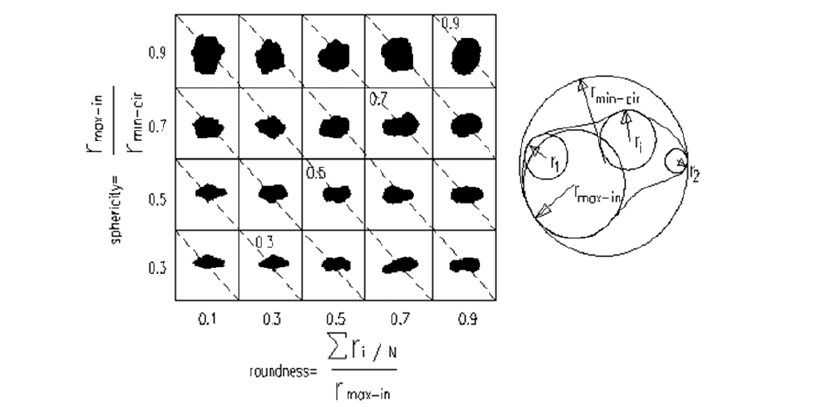
\includegraphics[width=0.5\linewidth]{figures//ch9/roundness.png}
    \caption{Roundness table \autocite{particle}}
    \label{fig:placeholder}
\end{figure}

\section{Consequences of dry sand mining}

\section{Recommendations and mitigation strategies}